% !TEX root = main.tex
%%%%%%%%%%%%%%%%%%%%%%%%%%%%%%%%%%%%%%%%%%%%%%%%%%%%%%%%%%%%%%%%%%%%%%%%%%%%%%%%
% Survival Analysis
%%%%%%%%%%%%%%%%%%%%%%%%%%%%%%%%%%%%%%%%%%%%%%%%%%%%%%%%%%%%%%%%%%%%%%%%%%%%%%%%
\section{Survival Analysis}
\label{section:survival}
\renewcommand{\pkg}[1]{\textsf{#1}}
\begin{figure*}
  \centering
  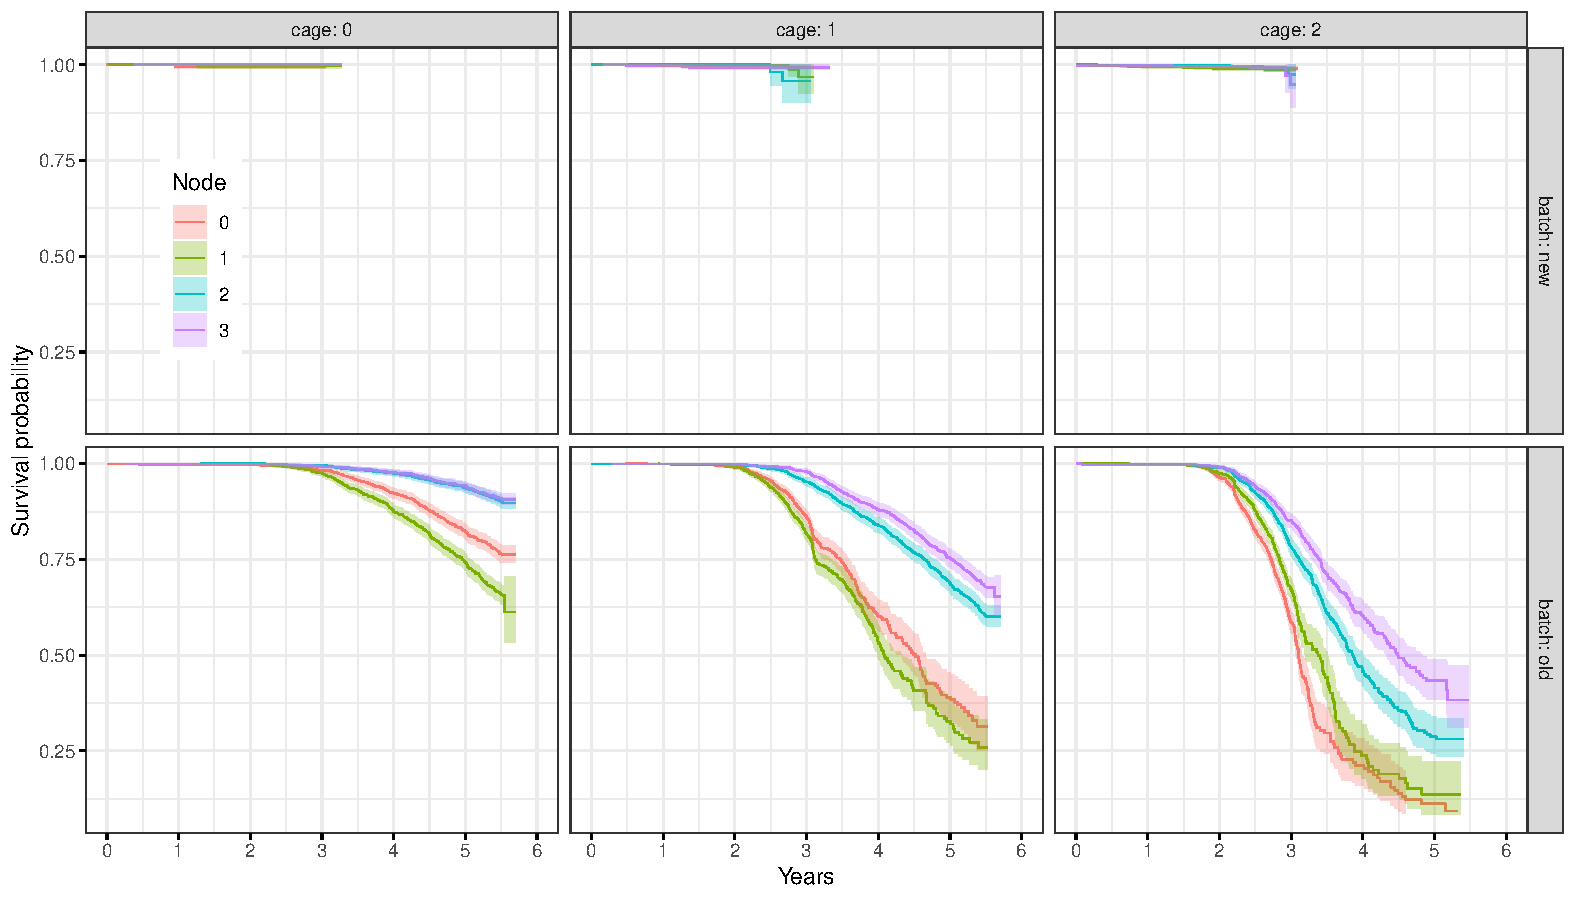
\includegraphics[width=7in]{figs/km_cage-node_a001.pdf}
  \caption{Comparison of the old and new batches, including survival
    differences based on {\tt cage} and {\tt node} GPU locations.}
  \label{fig:km-all-cage-node}
\end{figure*}
In this section we apply survival analysis methods (time to event
analysis), which use and combine information across the operational
lifetimes of all GPUs \cite{survival}. For these analyses, we take
apart the location string of each GPU into variables {\em col, row,
  cage, slot, and node} and study the influence of the locations on
the GPU life times. The construction of a GPU life time is more
complex than it initially appears because the units are observed only
at reboot time, because most units were proactively replaced to
prevent failure, and because some units continue in operation after
OTB and DBE events (when a second reboot may be successful).

A unit that experiences at least one OTB or DBE event and is removed
from the system is considered failed and its operation time until the
last seen time is taken as its life time. Although most failed units
experience one of these events at the last seen time, our definition
is not perfect because some units experience OTB or DBE events at a
time different from its last seen time. Such units were relatively few
so we consider this definition of life time as the most pragmatic.

A key concept in survival analysis is censoring, which is about using
information from study subjects whose exact failure times are not
available or that have not failed. This applies to our study because
of proactive GPU replacement before failure, because most units were
still in operation when the system was shut down, and also because
life spans were recorded only at inventory times. We use censoring
concepts on the proactive replacements and units still in operation at
the end. This allows us to use all of the GPU life time data,
including units that did not fail. But we ignore the inspection time
censoring, treating inventory times as exact failure times to reduce
the complexity of this analysis. We expect that because of the volume
of data and length of operation time, this would not make much
difference in our conclusions. However, we are making our data
publicly available and expect that others, especially in the survival
analysis community, will dive deeper.

Kaplan-Meier survival analysis (KM) starts with computing the
probability of survival beyond a given time. It is a nonparametric
technique that makes no specific failure model assumptions, such as
Weibull, Exponential, etc. The technique is able to use censored
observations and can also split the data into subpopulations to
compute separate survival curves.

If $T$ is the random variable of a GPU fail time, then its cumulative
distribution function $F(t) = Pr\{T < t\}$ gives the probability that
a GPU fails by duration $t$. The survival function is its complement
\begin{displaymath}
  S(t) = Pr\{T \geq t\} = 1 - F(t).
\end{displaymath}
It is the probability of being operational at duration $t$.  We use
the R packages \pkg{survival} and \pkg{survminer} for the KM analysis,
which is reported in Figure~\ref{fig:km-all-cage-node}. Within each
{\em batch}, separate survival curves are computed for each {\em cage}
by {\em node} combination. 

Another standard survival data methodology is a Cox proportional
hazards (CPH) regression analys, which can include covariates and
estimate relative risk based on the covariates
\cite{Cox1972,Harrell2015}. The CPH regression function takes the form
\begin{displaymath}
  h(t) = h_0(t)e^{b_1 x_1 + b_2 x_2 \ldots b_k x_k},
\end{displaymath}
where $x_i$ are covariates, $h_0(t)$ is the {\em baseline hazard}, and
the $b_i$ are coefficients that measure the impact of the
covariates. The quantity $e^{b_i}$ is the hazard ratio for covariate
$i$. Its interpretation 

That is, a base hazard rate multiplied by a function of
covariates. The key assumption in the CPH model is that the "hazards"
are multipliers on the "baseline hazard" but the estimate of the
baseline hazard is nonparametric, meaning it makes no specific
distributional assumption and just learns from the data (unlike
analyses that assume for example a Weibul or an exponential
model). The multiplicative assumption is that the hazard curves do not
cross and are multiples of each other. The multiplier is the *hazard
coefficient*. For example, if the baseline is *node0* and the *node2*
hazard is 2, then *node2* sees twice as many failures as *node0* on
average. 

For our comparison of hazards, we use as *covariates* all the unpacked
location variables, indicators whether the GPU has been moved, and our
notion of old and new GPUs based on first install date. Since many
GPUs experience time at more than one location, we use the longest
period location in this analysis. 

First, we do a univariate analysis for each covariate separately and
then we look at a multivariate view of this. Having multiple
covariates is called "multiple regression" as opposed to "multivariate
regression" reserved for cases with several response variables. The
univariate view is comparable to what would one see in a simple time
between failures analysis for a given population split. It can be
affected by sampling differences for other covariates. For example, if
the strongest effect is seen in a variable not used in a split and its
values are unevenly distributed across the split, its effect can leak
into the split. This is why we also do a multivariate analysis, where
the effect of each covariate is adjusted for all the other
covariates. 
 

\begin{figure}
  \centering
  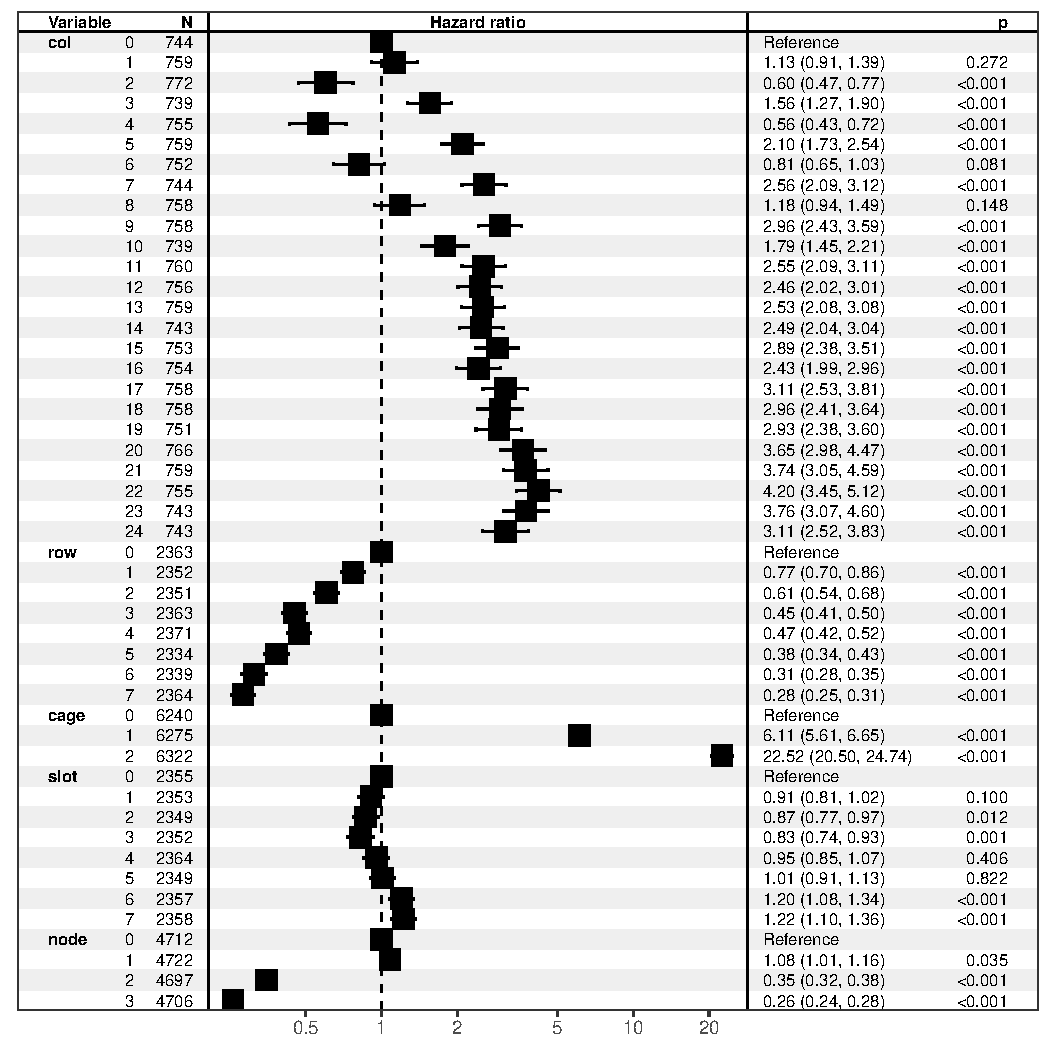
\includegraphics[width=0.8\columnwidth]{figs/cox_o001.pdf}
  \caption{GPU hazard ratios from Cox regression model on {\tt old}
    batch.}
\end{figure}
\begin{figure}
  \centering
  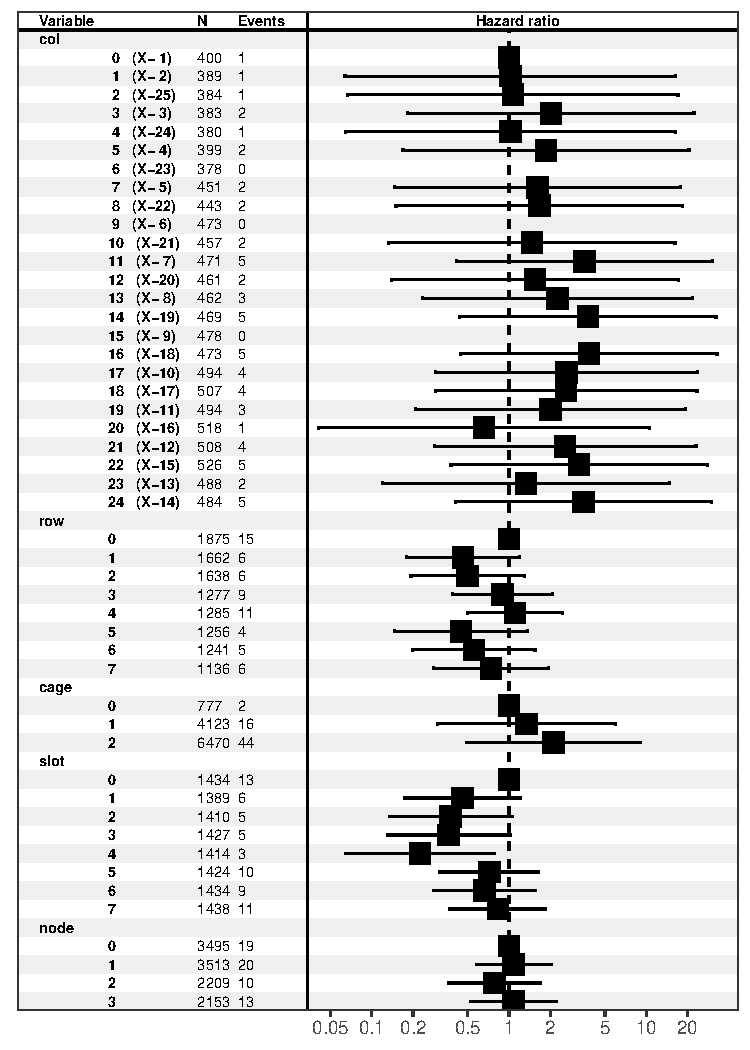
\includegraphics[width=0.8\columnwidth]{figs/cox_n001.pdf}
  \caption{GPU hazard ratios from Cox regression model on {\tt new}
    batch.}
\end{figure}

Higher numbered columns appear to have a higher (up to about 2x)
failure rate. There actually seems to be a hint of three groups that
have similar rates: 0-6 baseline, 7-16 are 1.5x baseline, and 17-24
are 2x baseline. 

Higher numbered rows tend to have a lower (up to about 0.5x) failure rate.

This seems surprisingly strong! Higher numbered cages have failure
rates 5x and 16x higher than cage = 0. In fact, this seems so strong
that its effect could be leaking into all other comparisons under
uneven sampling!

Not much difference between slots. They are all close to the baseline
slot0.

Interestingly, nodes 2 and 3 have half the failure rate of nodes 0 and
1. Is this related to the cage variable or is there a real location
effect?

Now the multivariate Cox regression analysis, where each factor is
adjusted for all the other factors. This can fix some uneven sampling
and multivariate dependence. 

The col groups persist and are even stronger. The row effect is also
stronger. The cage effect is out of this world! slot is still without
any effect. node effect also persists and is a bit stronger. 

Let’s separate the “old” and “new” batches of GPUs and run separate
Cox models. 
